\documentclass[11pt]{article}

\usepackage{hyperref}  % links
\usepackage{graphicx}  % images
\usepackage{listings}  % code
\usepackage{authblk}  % author info
\usepackage{biblatex}  % bibliography

\addbibresource{sources.bib}
\usepackage[utf8]{inputenc}

% Preamble
% Metadata
\title{Data Transfer in the Physical Layer Using LTE and Free-space Optical Communication as Guides}
\author{Daniel Opdahl}
\date{\today}

% Document Body
\begin{document}

\maketitle

\section{Abstract}

This paper will explore how data is transferred at the physical layer, touching on methods, issues, and overviews of infrastructure. I explore two broad mediums for physical data transfer in this paper: wireless electromagnetic data transmission, and optical data transmission. I give an overview of how data is transferred in each medium, as well as cover issues with transmitting data through that medium. I also explore a case study in each medium, discussing the finer details of each example.

\section{Introduction}

At its core, transferring data over a physical medium is simply communication. To talk about physical data transfer in the broadest sense is to talk about methods of human communication in the broadest sense. Semaphore, smoke signals, Morse code via heliograph, even basic verbal communication can all be considered physical data transfer. However, for the purposes of this paper,the scope of what physical data transfer is will be narrowed down to modern day inter-computer communication. Although much of what will be discussed here can be abstracted out to describe telegraph communication, beacon chain communication, and even homing pigeon communication, we will try to keep our focus around modern day architecture and methodology. 

In any data communication system, there are three components: the source, the transmission medium (or physical medium), and the destination. The source consists of the source machine and a transmitter. The source machine converts data into discrete digital signals and sends that to the transmitter to be converted into an analog signal. The transmitter sends the analog signal through the transmission medium to the destination. The transmission medium (e.g., a wire, the air, a cable) is simply something that can facilitate the propagation of the analog signal from source to destination. The destination consists of a receiver and the destination machine. The receiver receives data from the transmitter through the transmission medium in the form of an analog signal, converts that signal back into a discrete digital signal, which, in theory, should be the same as the original digital signal that the source machine passed to the transmitter. The receiver then passes the digital signal to the destination machine. Most often, both the receiver and transmitter consist of modems, and utilize hardware (such as an antenna or a photodetector) to do digital-to-analog conversion, or analog-to-digital conversion.

\section{Physical Layer Overview}

\begin{figure}[!htbp]
    \centering
    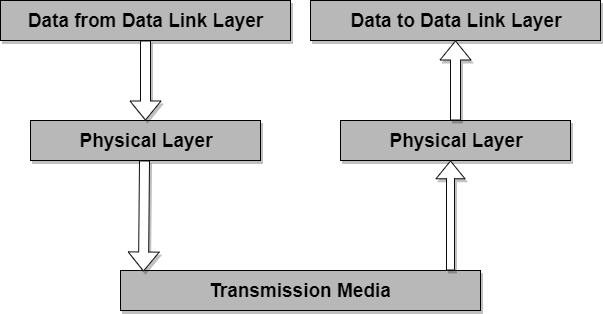
\includegraphics[width=0.4\textwidth]{PhysicalLayerOverview.png}
    \caption{An overview of the physical layer}
    \label{fig:PhysicalLayerOverview}
\end{figure}

In order for data to enter into the physical layer from the link layer, the data needs to take on a physical form, or signal. A signal is a physical representation of data, usually consisting of two modes that each represent a 0 or a 1, as almost all data transmission today is with binary bits. Signals can be a high and low voltage across an electrically conductive wire, a series of light pulses down a fiber optic cable, electromagnetic waves modulated based on frequency or amplitude, or any other physical representation that has two distinct states.

However, there is a fundamental problem with using a physical medium to transmit bits. Bits are binary, and as such, they are discrete, either a "one" or a "zero", "on" or "off". This means that to construct a signal of pure bits, the signal must be made of a series of discrete modes that represent the discrete values. This is most often done with a logic signal, a signal with only two possible values. Logic signals are connected to form line codes to construct digital signals. For the purposes of this paper, digital signals may only take on one of two values at most at any given time. Most commonly, digital signals are represented by two different voltages, one representing “off” or a “zero”, and one representing “on” or a “one”. Because a digital signal can only be one of two values at any time, small deviations from the specified voltages do not change the value that the digital signal encodes, because the deviations in voltages will always fall within the voltage band, by definition. 

\begin{figure}[!htbp]
    \centering
    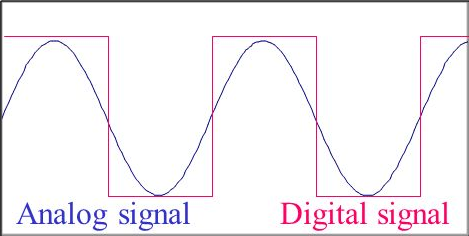
\includegraphics[width=0.4\textwidth]{analogdigitalsignalsForPaper.png}
    \caption{Analog signal vs digital signal}
    \label{fig:AnalogsignalvsDigitalsignal}
\end{figure}

Physical signals, on the other hand, are always analog signals, meaning that they are continuous, not discrete in value. This means that between an analog signal’s upper and lower bounds, it may take on one of any number of values at any time. Because of this, when an analog signal is represented by a varying physical phenomena (such as changing voltages), any deviation due to noise or error will manifest itself in the signal. This makes analog signals inherently prone to distorted signals, though usually devices that transmit analog signals select modes that are far enough apart relative to normal amounts of fluctuations, such that they are easy to differentiate. 

Because of the continuous value nature of analog signals, for any devices using analog signals to communicate, they must define thresholds for converting continuous analog signals into discrete digital signals and vice versa. These thresholds are defined by passbands and basebands.

A passband is a signal that corresponds to the “on” or “one” state. In reality, machines aren’t configured to only interpret one exact signal as a passband signal, but rather a range of signals. In most devices, especially ones that may receive data transmissions from multiple sources, for a passband signal to be received, it must first pass through a passband filter. A passband filter limits the range of frequencies that the device receives, allowing for the device to change what signal(s) are interpreted as passband signals.

A baseband is a signal that corresponds to the “off” or “zero” state. This means that baseband signals are transmitted without modulation, i.e., at, or near zero-frequency when compared with the highest frequency allowed. Similarly to passbands, there is typically not one exact signal that the machine will interpret as a baseband signal, but rather a range of signals. This range is called the baseband channel. Usually, the baseband signals that a machine receives are filtered out by the passband filter.

Any device using analog signals to communicate (i.e., any device that is transmitting over a physical medium) will necessarily need apparatuses to do digital-to-analog conversions and analog-to-digital conversions. The apparatuses that do these conversions are called modems (a portmanteau of “modulator-demodulator”). A receiving modem takes in an analog signal (usually a varying voltage or a series of light pulses) and, using a passband and a baseband, converts the analog signal into a digital signal or bitstream. A transmitting modem essentially does the opposite, taking a digital signal and converting it into an analog signal according to standardized frequencies between the two end systems, then sending that analog signal out through the transmission medium.

Finally, a line code is the pattern of voltages that both end systems agree upon to represent digital signals that are transmitted. A signal is line encoded before being transmitted through a physical medium. Most often, a line code is bipolar and consist of two opposite states, usually two voltages, one positive and one negative. For a line code to effectively facilitate communication between two devices, they must have synchronized clocks and agree upon the duration of a single bit of information within the signal. There are several methods to synchronize a transmitter and receiver, but the most common method is to allow the transmitter to transmit a line code at the rate they choose and to have the receiver measure the duration of time between "flips" of the signal, and adjust to the tempo the transmitter sets. Additionally, there are multiple different line codes that are commonly used, namely,  unipolar, polar, bipolar, and Manchester code. Unipolar encoding uses a positive voltage (or light pulse, etc.) to represent a 1, and no voltage (or absence of light, etc.) to represent a 0. Polar encoding uses a positive voltage (or light pulse, etc.) to represent a 1, and an equal but opposite negative voltage (or pulse of light of a different wavelength, etc.) to represent a 0. In bipolar encoding, an alternate mark inversion (AMI) is used, meaning an absence of voltage (or absence of light, etc.) represents a 0, and an alternating positive and negative voltage represents a 1. This promotes transmission integrity because if a receiver receives two positive or two negative voltages in a row, something has gone wrong. Manchester code assigns each bit to be either a positive voltage then negative (or zero) voltage in one time period to represent one bit, or a negative voltage then a positive (or zero) voltage in one time period to represent the other bit. The benefit of Manchester code is that it is self-clocking, and does not require the clocks of the transmitter and receiver to be synchronized.

\begin{figure}[!htbp]
    \centering
    \begin{minipage}{0.45\textwidth}
        \centering
        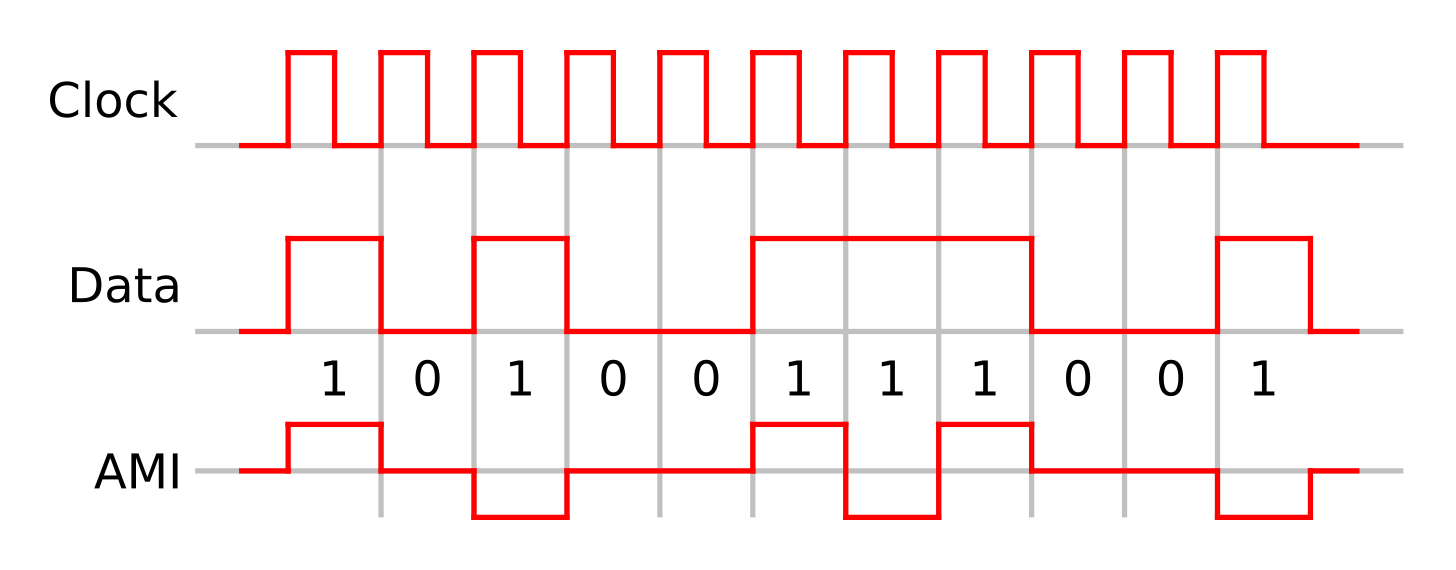
\includegraphics[width=0.9\textwidth]{bipolarencoding.png}
        \caption{Bipolar encoding}
        \label{fig:bipolarencoding}
    \end{minipage}
    \begin{minipage}{0.45\textwidth}
        \centering
        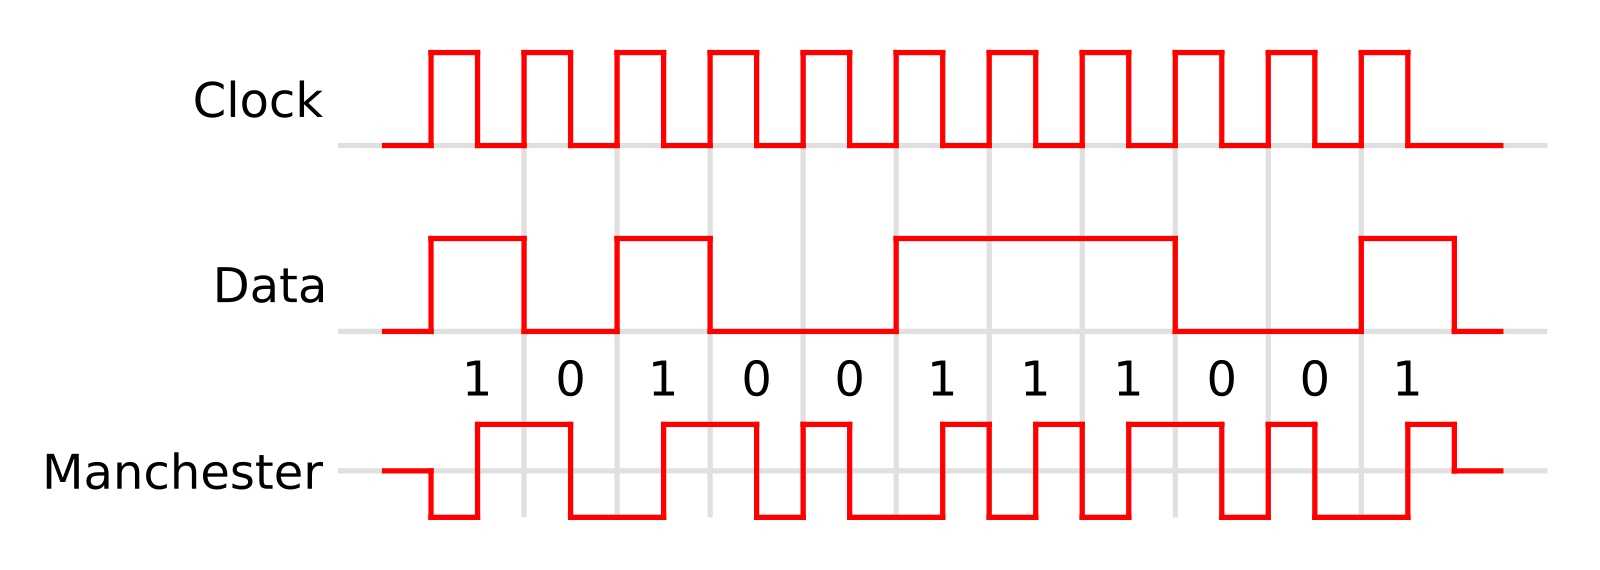
\includegraphics[width=0.9\textwidth]{manchesterencoding.png}
        \caption{Manchester encoding}
        \label{fig:manchesterencoding}
    \end{minipage}
\end{figure}

\section{Wireless Electromagnetic Data Transfer}

\subsection{Basics of Electromagnetic Waves}

In a classical physical sense, electromagnetic waves are synchronized oscillations of electric and magnetic fields that propagate through space and carry electromagnetic energy. Electromagnetic waves can be classified according to their wavelength or oscillation frequency, having the relationship \begin{math} \lambda = \frac{c}{f} \end{math}, where \begin{math} \lambda \end{math} is the wavelength, \begin{math} c \end{math} is the speed of light (in a given medium), and \begin{math} f \end{math} is the frequency. For the purposes of this paper, this definition of electromagnetic waves will suffice, and we will not need to touch on quantum mechanical definitions of electromagnetic radiation. 

Electromagnetic waves propagate through space, without the need of a transmission medium, and in fact can be impeded by physical objects, depending on the waves’ frequency and the object's physical properties. 
All data transfer using electromagnetism utilizes electromagnetic waves. In order for an electromagnetic wave to transmit data, it must be modulated. Modulation is the process of varying one or more of the properties of a wave in order to create two distinct modes that can represent either value of a bit (“zero” or “one”). For example, in radio broadcasting, frequency modulation is often used, which (in the simplest case) varies the frequency of the outgoing modulating signal in order to create a high frequency signal that corresponds with a “one” and a low (or no) frequency signal that corresponds with a “zero”.Since the invention of the radio, however, there have been multiple new ways invented to modulate electromagnetic waves to carry data, such as single-sideband modulation, which is often used in Wi-Fi networks, but is beyond the scope of this paper.

\subsection{How an Antenna Transmits Data}

All wireless electromagnetic communication requires the use of an antenna. An antenna is the interface between electromagnetic waves and electrical currents in transmitters and receivers. It is made of an array of conductors that are linked in a circuit with a transmitter and a receiver. For an electromagnetic wave to be created, a transmitter needs to supply an electric current or voltage to the antenna, and as the electrons undergo acceleration due to the applied electrical current or voltage, they produce changing electric and magnetic fields, otherwise known as an electromagnetic wave. Similarly, for an antenna to pick up an electromagnetic wave, an electromagnetic wave needs to hit an antenna, which will create very small changes in current or voltage inside the conductive antenna, which can then be picked up by a receiver. The amount of current or voltage that is input into an antenna modulates the electromagnetic wave, allowing for the transfer of data.

\subsection{Issues}

There can be many issues with transmitting data with electromagnetic waves such as fading, and path loss. There are other issues, but they will not be explored here. Fading is the variation of the intensity and clarity of an electromagnetic wave over time and distance. Oftentimes, this is effectively a random process and leads to corrupted data without recourse. Path loss is the weakening of the intensity and clarity of an electromagnetic wave over time and distance, leading to more ambiguous data transfer. Path loss is distinct from fading in that path loss is the reduction in strength of the signal, whereas fading is an increase in random variations introduced into the signal by environmental factors. 

\subsection{LTE}

Long-Term Evolution (LTE) is a wireless standard for data transmission, usually used by mobile devices. It operates on several frequencies, usually from around 500 MHz to 3500 MHz, with bandwidths ranging from 1.4 MHz to 20 MHz in range. LTE uses Orthogonal frequency division multiplexing (OFDM) that uses a large number of narrowband sub-carriers to multi-carrier transmission. This allows LTE to transmit data over multiple frequencies at multiple rates. Each user is allocated a number of “resource blocks”, and the more resource blocks a user receives and the higher the frequency bands of those blocks, the higher the bit rate will be for the user. Users are allocated frequency bands based on scheduling mechanisms that are beyond the scope of this paper.Because of the dynamic way frequency bands are assigned to users, LTE can offer download speeds of up to 300Mbps.

\begin{figure}[!htbp]
    \centering
    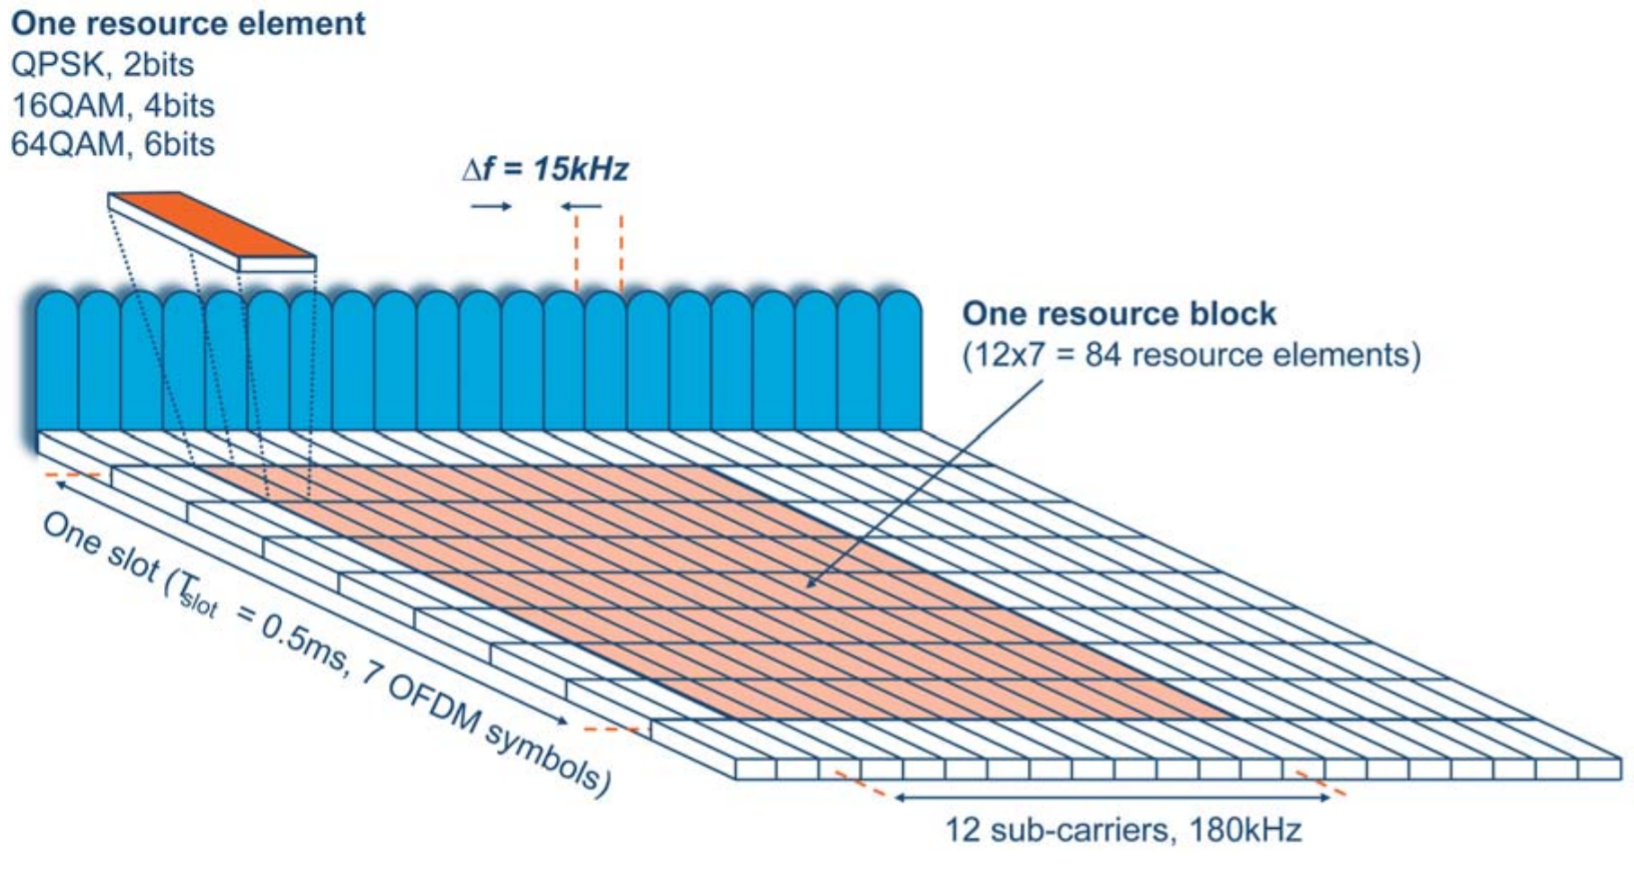
\includegraphics[width=0.4\textwidth]{OFDMDiagramForPaper.png}
    \caption{LTE use of orthogonal frequency division multiplexing}
    \label{fig:OFDMDiagram}

\end{figure}

\section{Optical Data Transfer}

In contrast to electromagnetic waves, in a classical physical sense, optical data transfer is done with packets of light called photons. For the purposes of this paper, photons can be thought of as particles of light that have a frequency (color), and travel at the speed of light in whatever medium they are travelling. As with any other method of physical data transfer, in order for a packet of photons to be able to transmit data, a signal has to be modulated. However, in optical data transfer, it is not necessarily the frequency of the photons that is modulated, though that is a valid modulation method. Often, it is the absence of light that is used in modulation to create two distinct modes, though this does require the transmitter and receiver to agree on the length of time for a single bit to be transmitted. For example, a transmitter and receiver could define the time length for transmission of one bit to be one second, so one second of no photons means a “zero” and one second of photons means a “one”. 

Optical data transfer, unlike wireless electromagnetic data transfer, is not effective when used omnidirectionally. In order to direct photons to their intended destination, most of the time optical fiber is used. Optical fibers are not like a typical metal wire that carry signals via varying voltages. Optical fibers are tubes of glass that exhibit total internal reflection, meaning that photons travel down the tube without escaping until the end of the tube. There are other methods of optical data transfer that do not employ optical fibers (such as high-intensity lasers), but they are usually not used terrestrially, as physical interference makes this method impractical. 

Additionally, transmitters and receivers using optical data transfer can use wave division multiplexing to vastly increase the throughput through optical fibers. Wave division multiplexing is the process of multiplexing, or combining, several optical signals into one signal and sending that signal through the optical fiber. This allows not only for a large increase in the potential throughput of the fiber, but also for multidirectional simultaneous data transfer. 

\subsection{Transmitters}

Optical transmitters are devices that send light across a medium (usually a fiber optic cable). Specifically, these devices are usually either LEDs or laser diodes. Often, laser diodes are directly modulated, meaning that light emission in the device is controlled directly by the supplied current. Usually this either means that there is either a threshold current (where the laser will be on if the current is above the threshold, and off if the current is below), or that the frequency of the light emitted by the laser will continually change in proportion to the changing current. These two methods represent a digital signal being transmitted optically, and an analog signal being transmitted optically, respectively. 

\subsection{Receivers}

The main component of an optical receiver is a photodetector, a device that detects incoming light via the photoelectric effect. The photoelectric effect, put simply, is when light of a certain frequency strikes a certain material, that material will release electrons, creating a small current. An optical receiver will detect a current via the photodetector when light is coming in through the fiber optic cable, thus demodulating the signal. 

\subsection{Free-space Optical Communication}

Free-space optical communication is a method of optical data transmission that uses free space as the transmission medium. Using free space (e.g., air, outer space, etc) as a transition medium inherently presents several problems, however. First of all, if using lasers to optically communicate, the transmitter’s beam has to hit the photodetector. Aiming the laser precisely like this is simple at short distances, but gets exponentially more difficult to aim precisely the farter away the two end systems are due to the inverse square law. Additionally, oftentimes free-space optical communication is seen as a solution when a transmitter and receiver are not stationary and a fiber optic cable is not feasible. This adds another level of difficulty when designing mechanisms to aim a laser precisely. Additionally, the physical properties of the free space such as fog, rain, light pollution, smog, or general atmospheric absorption may cause attenuation or distortion of the signal. There have been some solutions to these issues such as using more intense beams, or using multiple transmitters and receivers.

In recent years, satellites in space have been using free-space optical communication, as it presents an elegant solution for inter-satellite communication. Many of the issues with optical data transmission in free space are nullified by being in space, however technical challenges still exist, and the world is still in the early stages of implementing this technology. The first gigabit laser-based communication commenced operation on November 28, 2014, named the European Data Relay System by the European Space Agency. It is still operational and is used daily. NASA has implemented several demonstrations of free-space optical communication, notably aboard the MESSENGER spacecraft. The spacecraft was able to communicate over a distance of 24 million km in 2004. NASA also successfully beamed an image of the Mona Lisa to the Lunar Reconnaissance Orbiter over a distance of 390,000 km. In the commercial realm, Space X’s Starlink project is attempting to provide satellite global broadband coverage using inter-satellite optical laser communication between several hundred to thousand satellites. 

\nocite{*}
\printbibliography
\end{document}
